\documentclass[tikz,border=4pt]{standalone}
\usepackage{tikz}
\usetikzlibrary{arrows.meta,patterns}
\definecolor{nebula}{HTML}{6366F1}
\definecolor{spark}{HTML}{14B8A6}
\begin{document}
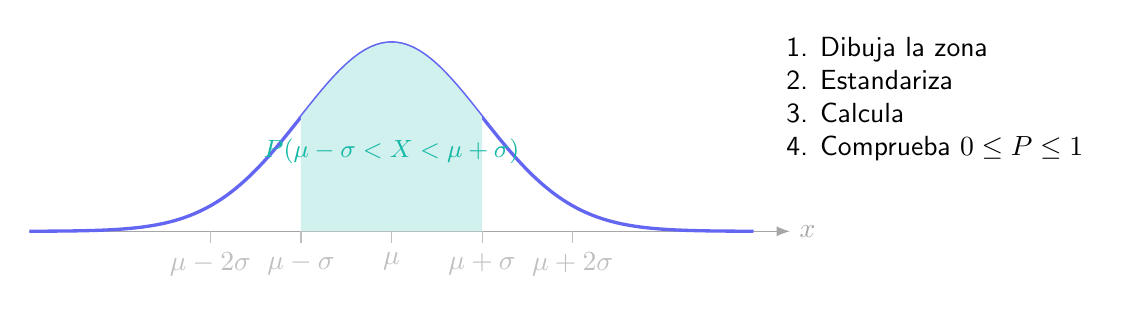
\begin{tikzpicture}[x=1.15cm,y=6cm,font=\sffamily,>=Latex]
  \draw[->,gray!70] (-4,0)--(4.4,0) node[right] {$x$};
  \draw[domain=-4:4,samples=180,very thick,nebula] plot (\x,{0.3989*exp(-\x*\x/2)});
  \fill[spark!20,domain=-1:1,samples=90] plot (\x,{0.3989*exp(-\x*\x/2)}) -- (1,0)--(-1,0)--cycle;
  \foreach \x/\lab in {-2/$\mu-2\sigma$,-1/$\mu-\sigma$,0/$\mu$,1/$\mu+\sigma$,2/$\mu+2\sigma$}{\draw[gray!50](\x,0)--(\x,-.025)node[below]{\lab};}
  \node[spark] at (0,.17) {\small $P(\mu-\sigma<X<\mu+\sigma)$};
  \node[align=left] at (6,.28) {1. Dibuja la zona\\2. Estandariza\\3. Calcula\\4. Comprueba $0\leq P\leq1$};
\end{tikzpicture}
\end{document}
